%%%%%%%%%%%%%%%%%%%%%%%%%%%%%%%%%%%%%%%%%
% Journal Article
% LaTeX Template
% Version 1.3 (9/9/13)
%
% This template has been downloaded from:
% http://www.LaTeXTemplates.com
%
% Original author:
% Frits Wenneker (http://www.howtotex.com)
%
% License:
% CC BY-NC-SA 3.0 (http://creativecommons.org/licenses/by-nc-sa/3.0/)
%
%%%%%%%%%%%%%%%%%%%%%%%%%%%%%%%%%%%%%%%%%

%----------------------------------------------------------------------------------------
%	PACKAGES AND OTHER DOCUMENT CONFIGURATIONS
%----------------------------------------------------------------------------------------

\documentclass{article}

%\documentclass{aastex}  % version 5.0 or prior
%\usepackage{natbib}



\usepackage{graphicx}
\usepackage{lipsum} % Package to generate dummy text throughout this template
%\usepackage[sc]{mathpazo} % Use the Palatino font
\usepackage[T1]{fontenc} % Use 8-bit encoding that has 256 glyphs
\linespread{1.05} % Line spacing - Palatino needs more space between lines
\usepackage{microtype} % Slightly tweak font spacing for aesthetics

\usepackage[margin=1in,columnsep=20pt]{geometry} % Document margins
\usepackage{multicol} % Used for the two-column layout of the document
\usepackage[hang, small,labelfont=bf,up,textfont=it,up]{caption} % Custom captions under/above floats in tables or figures
\usepackage{booktabs} % Horizontal rules in tables
\usepackage{float} % Required for tables and figures in the multi-column environment - they need to be placed in specific locations with the [H] (e.g. \begin{table}[H])
\usepackage{hyperref} % For hyperlinks in the PDF
\usepackage{subcaption}

\usepackage{lettrine} % The lettrine is the first enlarged letter at the beginning of the text
\usepackage{paralist} % Used for the compactitem environment which makes bullet points with less space between them
\usepackage{amsmath}
\usepackage{abstract} % Allows abstract customization
\renewcommand{\abstractnamefont}{\normalfont\bfseries} % Set the "Abstract" text to bold
\renewcommand{\abstracttextfont}{\normalfont\small\itshape} % Set the abstract itself to small italic text

\usepackage{titlesec} % Allows customization of titles
%\renewcommand\thesection{\Roman{section}} % Roman numerals for the sections
%\renewcommand\thesubsection{\Roman{subsection}} % Roman numerals for subsections
%\renewcommand\thesubsubsection{\Alph{subsubsection}} % Roman numerals for subsections
\titleformat{\section}[block]{\LARGE\scshape}{\thesection}{1em}{} % Change the look of the section titles
\titleformat{\subsection}[block]{\Large\scshape}{\thesubsection}{1em}{} % Change the look of the section titles
\titleformat{\subsubsection}[block]{\large\scshape}{\thesubsubsection}{1em}{} % Change the look of the section titles

\usepackage{fancyhdr} % Headers and footers
\pagestyle{fancy} % All pages have headers and footers
\fancyhead{} % Blank out the default header
\fancyfoot{} % Blank out the default footer
\fancyhead[C]{Montana State University \quad $\bullet$ \quad CSCI 466 Artificial Intelligence \quad $\bullet$ \quad Group 21} % Custom header text
\fancyfoot[RO,LE]{\thepage} % Custom footer text

\newcommand{\ve}[1]{\boldsymbol{\mathbf{#1}}}

\title{\vspace{-15mm}\fontsize{24pt}{10pt}\selectfont\textbf{CSCI 446 Artificial Intelligence \\[2mm] Project 3 Design Report} } % Article title
\date{\today}
\author{
\large
\textsc{Roy Smart} \and \textsc{Nevin Leh} \and \textsc{Brian Marsh}\\[2mm] % Your name
}


%----------------------------------------------------------------------------------------

\begin{document}

	\maketitle % Insert title
	\thispagestyle{fancy} % All pages have headers and footers
	\normalsize

	\section{Introduction}
	Introduce Machine Learning Algorithm (MLA)!!!!
	Explain classification problem!!!
	\section{Datasets}
		\subsection{Dataset Representation}
			We will define a \textit{datum} to be a vector consisting of the class as the zeroth element and the associated attributes as the rest of the elements. Classes and attributes will be represented by an integer. Continuous data will be binned before it is inserted into each datum. The resolution of the bins will be a variable that will have to be tuned. Each dataset will be represented as a vector of datums.
		\subsection{Data Imputation}
			Imputation is the process of approximating missing values in the datasets. 
			To our knowledge there is only one dataset that has real missing values: the Wisconsin Breast Cancer Database. 
			The 1984 United States Congressional Voting Records Database appears to have missing values, but these can actually be interpreted as a stance on a particular issue. 
			Since the breast cancer database has a small proportion of missing values, it is appropriate to simply eliminate datums with missing values. 
			The authors assert that trying to train a MLA with imputed values would only create unnecessary bias in the network.
			
			However, it is a common real-world problem to attempt to classify an unknown, incomplete datum, therefore we will perform imputation on the validation datasets. 
			To approximate the missing values we will first try a hot-deck imputation, where missing attribute values of a given datum are constructed by selecting a random member of that datum's class and copying the value of the attribute. 
			If the hot-deck is unsuccessful, we will attempt to fill in the missing values using a regression model developed in \textit{Mathematica}.
		\subsection{Cross-validation}
			To partition the full datasets into test and training datasets, we will use 10-fold cross validation. 
			This method partitions the data into ten \textit{folds} and uses one fold for testing data and the remaining nine folds for the training dataset. 
			This process is repeated nine more times until every fold has been used as a test dataset. 
			We selected this method because it will allow the convergence measurement described in Section \ref{convergence} to be applied over a larger range, which allows us to measure the rate of convergence for each MLA more accurately.
	\section{Machine Learning Algorithms}
		\subsection{$k$-Nearest Neighbors}
		\subsection{Naive Bayes}
			\label{nbw}
			\subsubsection{Description}
				\label{nb_des}
				\textit{Naive Bayes} uses the principle of Bayesian learning to solve the classification problem. This algorithm is said to be naive because it considers the attributes to be conditionally independent when performing classifications. Under this scheme, the probability distribution of each class $C$ is given the set of attributes $x_1,...,x_n$ is written by Russell and Norvig as
				\begin{equation*}
					\ve{P}(C|x_1,...,x_n) = \alpha \ve{P}(C) \prod_i \ve{P}(x_i| C) \label{nb_pd}
				\end{equation*}
				where, using the maximum likelihood hypothesis, $\ve{P}(C)$ prior probability of the class $C$ in the training dataset, $\ve{P}(x_i|C)$ is the likelihood of attribute $x_i$ given $C$, and $\alpha$ is a normalization constant. To find $\ve{P}(C)$ the we simply say it is equal to the proportion of $C$ observed in the training dataset. Likewise we can calculate the likelihood using
				\begin{equation*}
					P(a|b) = \frac{P(a \land b)}{P(b)}
				\end{equation*}
				where the probabilities are calculated using the number of occurrences in the training dataset. In this way, naive Bayes can make predictions using only the probability ratios constructed from the training dataset. The probability distribution in the naive Bayes algorithm can be viewed as a Bayesian network, shown in Figure \ref{nb} where each attribute is only connected to the class, and there are no relationships between attributes.
				\begin{figure}[h]
					\centering
					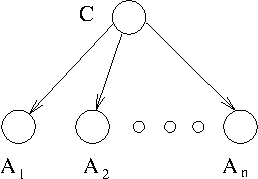
\includegraphics[width=0.3\textwidth]{fig/nb}
					\caption{An example of a Bayesian network for naive Bayes. The root $C$ is the class, the leaves $A_1,...,A_n$ are the attributes \cite{Friedman1997}}
					\label{nb}
				\end{figure}
			\subsubsection{Design Implications}
				This algorithm should be very straightforward to implement. During the training phase, we simply loop through the dataset and tally how many times each class takes on every value of each attribute. During the testing phase, the algorithm uses the equations described in Section \ref{nb_des} to select the most probable class.
		\subsection{TAN}
			\subsubsection{Description}
				\textit{Tree-Augmented Naive Bayes} (TAN) is an extension to the naive Bayes algorithm described in Section \ref{nbw}. First described by \cite{Friedman1997} TAN relaxes the assumption that the attributes are conditionally independent and allows each attribute to depend on only one other attribute. It accomplishes this by constructing a fully-connected, undirected graph out of the attributes in the Bayesian network for the naive Bayes algorithm (Figure \ref{nb}). TAN then assigns a weight to each connection in the graph using the \textit{mutual information function}, given by
				\begin{equation*}
					I_P(\ve{X};\ve{Y}) = \sum_{\ve{x},\ve{y}} P(\ve{x},\ve{y}) \log \left( \frac{P(\ve{x},\ve{y})}{P(\ve{x})P(\ve{y})} \right).
				\end{equation*}
				Applying the this weight to the edges allows us to construct a minimum spanning tree of the graph. We can then make the spanning tree directed by choosing a root node and setting the direction of all edges to be outward from it. The result is exemplified in Figure \ref{tan}.
				\begin{figure}[h]
					\centering
					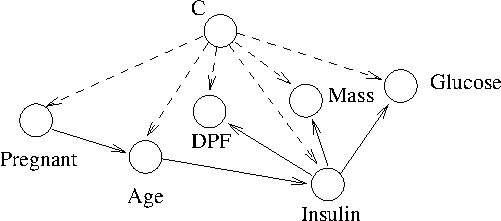
\includegraphics{fig/tan}
					\caption{An example of the directed minimum spanning tree produced by TAN. Dashed lines represent the original naive Bayes representation and the solid lines represent the spanning tree \cite{Friedman1997}.}
					\label{tan}
				\end{figure} 
			\subsubsection{Design Implications}
		\subsection{ID3}
	\section{Software Architecture}
	\section{Experiment Design}
		\subsection{Algorithm Accuracy}
			\subsubsection{Precision}
			\subsubsection{Recall}
			\subsubsection{Confusion}
		\subsection{Algorithm Time-Complexity}
		\subsection{Algorithm Convergence}
			\label{convergence}

	\begin{equation*}
		H(S) = \sum_{i=1}^{n} \left( -p_i \log_2 p_i \right)
	\end{equation*}

	%\bibliographystyle{apj}
	\bibliographystyle{apalike}	
	\bibliography{sources}
\end{document}
